% version 1.00, date 23/02/16, auteur Matthieu Martins-Baltar
\subsection{Fonctionnalité 2}
La fonctionnalité 2 du système devra permettre les opérations conventionnelles de gestion individuelle comme la création d'un établissement dans le système, la modification des
caractéristiques le concernant, la suppression d'un établissement. La figure \ref{creationDunEtablissement} présentera le diagramme de cas d'utilisation concernant la création d'un établissement.\\
 Comme pour un bénévole, la suppression devra être logique et non physique de façon à ne pas perdre l'historique des actions effectuées dans cet établissement sachant que la disparition peut être temporaire en fonction de l'ouverture et la fermeture de classes. \\

\begin{figure}[H]
	\centering
	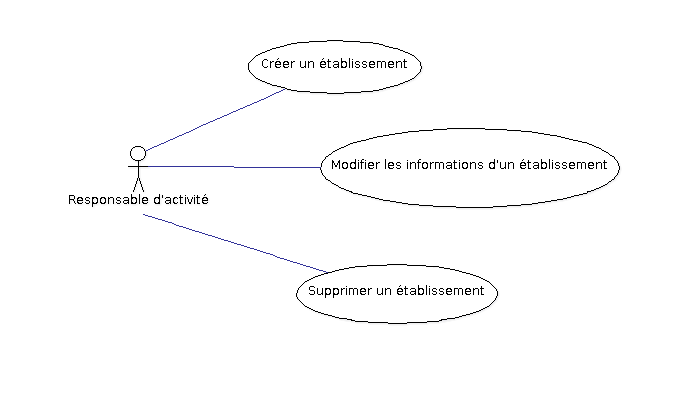
\includegraphics[scale=0.4]{images/casDUtilisation/fonctionnalite2Etablissement.png}
	 \caption{Cas d'utilisation~: créer un établissement}
	 \label{creationDunEtablissement}
\end{figure}


Les informations associées à un établissement sont :
\begin{itemize}
\item sa ville de rattachement (unique), 
\item son nom lorsqu'il existe (attention dans la même ville il peut y avoir une école élémentaire et une école maternelle sans nom spécifique), 
\item son adresse,
\item son code postal,
\item le responsable de l'établissement, 
\item le contact plaidoyers (facultatif),
\item le contact frimousse (facultatif),
\item le contact pour les activités ponctuelles (facultatif),
\item le numéro de téléphone fixe de l'établissement, 
\item la ou les adresse(s) électronique(s) de l'établissement (attention toutes les adresses électroniques ne sont pas forcément celles définies par le rectorat notamment pour les établissements privés ou pour les centres de loisirs), 
\item le nom, le numéro de téléphone fixe et/ou portable de l'enseignant demandant une intervention, son adresse électronique (toutes ces informations ne sont pas forcément disponibles). Il peut y avoir plusieurs enseignants pour la même classe (donc plusieurs contacts possibles).
\item sa localisation géographique (Latitude-Longitude en WGS84) si elle est disponible.
\item son type (enseignement ou centre de loisirs)
\\
\end{itemize}
Les enseignements ont un UAI et un type d'enseignement (l'enseignement supérieur, les lycées, les collèges, les écoles élémentaires et maternelles). \\
Les centres de loisirs ont un type de centre (maternelle, élémentaire et adolescent). 
